\documentclass{article}
\usepackage{geometry}
\usepackage{hyperref}
\usepackage{fancyhdr}  
\usepackage{graphicx}

\geometry{
  top=1in,
  bottom=1.5in,
  left=1.25in,
  right=1.25in
}

\title{Rapport de projet IA41 - Rasende Roboter}
\author{SENGEL Noé, POURCINE Mattéo, FLEURET Gabriel}
\date{\today}


\begin{document}

\maketitle

\tableofcontents
\newpage
\section{Mise en contexte}
Le but de ce projet est de mettre en application les différents algorithmes vu en cours pendant le semestre d'automne 2023 en \textbf{IA41} (\href{https://fr.wikipedia.org/wiki/Algorithme_de_parcours_en_largeur}{Breadth-First Search}, \href
{	https://en.wikipedia.org/wiki/A*_search_algorithm}{A*}, \href{https://en.wikipedia.org/wiki/Depth-first_search}{Depth-first search}).\\
Ces algorithmes vont être appliqués sur un jeu de société allemand, \href{https://fr.wikipedia.org/wiki/Ricochet_Robots}{\textbf{Rasende Roboter}} ou \href{https://fr.wikipedia.org/wiki/Ricochet_Robots}{Ricochet Robots} en français, créé en 1999 par \href{https://fr.wikipedia.org/wiki/Alex_Randolph}{Alex Randolph}.\\
\\
Nous étions trois à réaliser ce projet. Pour nous permettre de s'organiser au mieux, nous avons choisit de faire un répertoire \href{https://github.com/Glenrunc/IA41_Rasende_Roboter}{\textbf {Github}}. Notre raisonnement a été assez simple concernant l'approche du projet. Nous avons décidé d'implémenter premièrement le jeu pour ensuite y incorporer les algorithmes de résolution.\\\\
Plusieurs sources ont été utiles à la réalisation de ces travaux. Vous les trouverez en fin de rapport.
\section{Implémentation du jeu}
Nous avons fait le choix de prendre la première version du jeu. En effet une autre est apparu en 2003, qui ajoutait un robot noir, une case mission multicolore et des agencements de mur différents.
\subsection{Règles du jeu}
Les règles sont assez simple. Le joueur dispose d'un plateau de 16x16 cases. Sur celui-ci est diposé 4 robots de couleurs différentes (rouge, vert, bleu et jaune) et des jetons "missions". Une case centrale permet d'afficher la mission a atteindre par le robot de la couleur de celle-ci.\\ Le but est pour le joueur d'atteindre la mission avec le robot de la couleur correspondante en un minimum de coup et un minimum de temps. Pour cela il peut déplacer tous les robots comme il le souhaite.\\\\
\begin{figure}[h]
  \centering  
  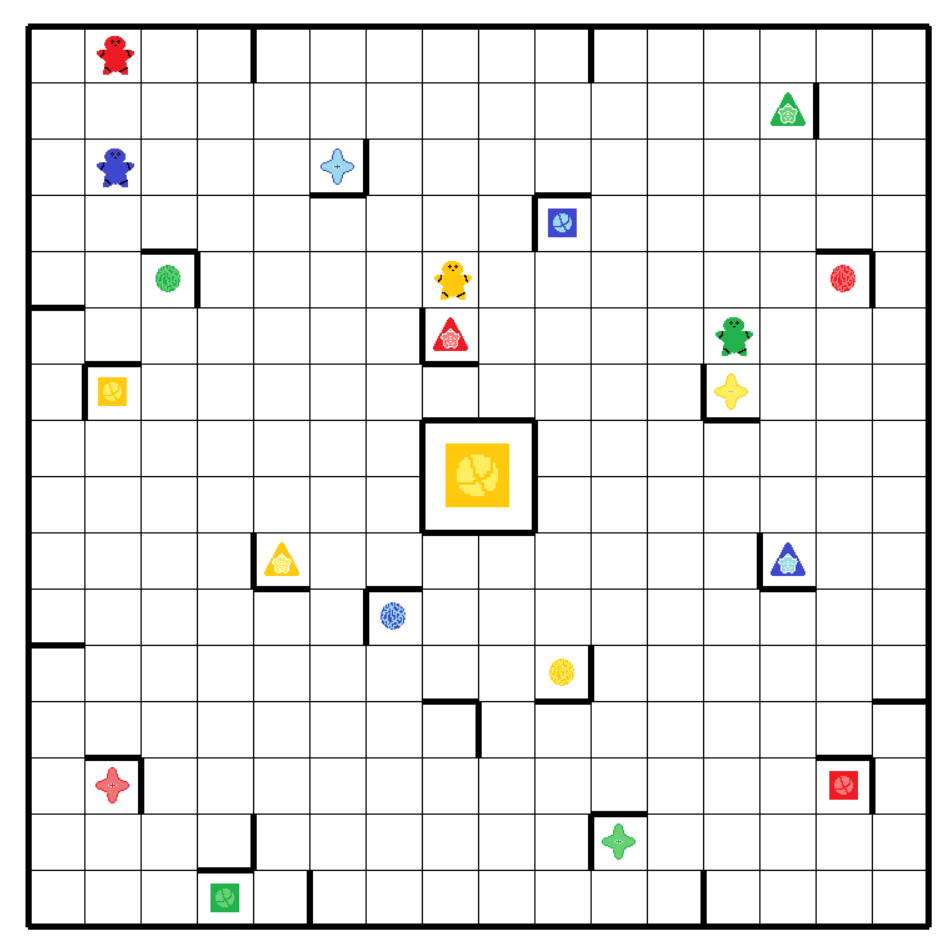
\includegraphics[width=0.5\textwidth]{map_rasende.png}  
  \caption{Image du plateau de jeu "Rasende Roboter"} 
  \label{fig:Plateau}  
\end{figure}
\\
Les déplacements sont assez simple également. Les robots ne peuvent suivre que 4 directions (haut, bas, gauche, droite). De plus une fois qu'une direction est prise, le robot en question ne s'arrête que lorsqu'il croise un mur ou un autre robot.\\\\Chaque partie commence par le tirage d'une mission. Une fois la mission choisit, un compte à rebourt est lancé. Pendant ce temps les différents joueurs analyse la position de chaque robot et essaye, dans leur tête, de trouver un moyen de résoudre le problème. Pour faciliter la compréhension, si on regarde la Figure 1, le robot jaune doit atteindre la cible afficher au centre du plateau. Ici elle se situe aux coordonnées (7,2).\\\\
Si un joueur à une solution, il fait signe et donne sa réponse. Si elle est bonne, il gagne, sinon les autres tentent de résoudre le problème.
\subsection{Choix et explications de notre implémentation}
Le but du projet étant d'implémenter différents algorithmes de résolutions, il nous ait paru évident de modifier certains points du jeu.\\\\Dans la version physique, le jeu se joue à plusieurs, chacun pour soi. Nous avons décider que notre jeu pouvait se jouer seul ou à plusieurs contre les algorithmes de résolutions. Ainsi le but de chaque partie est de résoudre le problème en moins de coup possible certes, mais surtout en moins de coup que l'intelligence artificielle.\\\\Lorsque qu'on arrive sur le jeu, on peut choisir le nombre de  manches que l'on veut jouer. A la fin de celles-ci on compte le nombre de manches gagnées contre l'IA. Si ce nombre est supérieur à celui du nombre de manche perdu, on gagne la partie, sinon on perd.\\\\On peut également choisir de "Reset" la manche si on voit que l'on bloque. Un mode revisionnage à été implémenté pour voir les coups effectués par l'IA. Ce mode est uniquement disponible lorsque la manche est terminée. Enfin un boutton abandon permet de passer à la manche suivante et met automatiquement l'IA vainqueur.\\\\
Au niveau de l'ergonomie de jeu. Il se joue uniquement grâce à une souris ou un pavé tactile. Lorsque l'on clique sur un robot, un chemin s'affiche pour aider le joueur à voir les cases atteignables. Ensuite il peu cliquer sur les différents chemin possible pour déplacer le robot. 
\begin{figure}[h]
  \centering  
  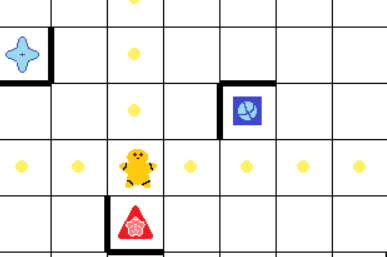
\includegraphics[width=0.5\textwidth]{deplacement.png}  
  \caption{Exemple de déplacement du robot jaune} 
  \label{fig:Plateau}  
\end{figure}
\section{Approche orientée objet}
Pour ce qui est de l'implémentation du jeu uniquement, nous vous détailleront certaines méthodes servant aux algorithmes de résolution. Mais pour le reste, nous avons décidé de faire uniquement un diagramme de classe pour rendre plus visuel nos explications. 
\begin{figure}[h]
  \centering  
  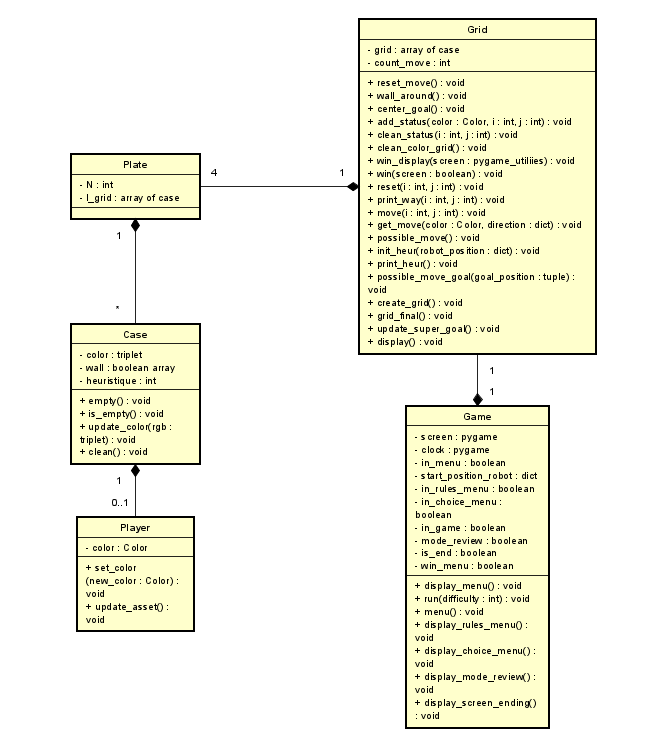
\includegraphics[width=1\textwidth]{diagram_class.png}  
  \caption{Diagramme de classe du jeu Rasende Roboter} 
  \label{fig:Plateau}  
\end{figure}

\end{document}
